\documentclass{standalone}

\usepackage[euler-digits]{eulervm}
\usepackage{amssymb}

\usepackage{tikz}
\tikzset{every node/.style={circle,draw,minimum size=6mm,inner sep=0pt}}
\tikzset{t/.style={rectangle}}

\begin{document}
    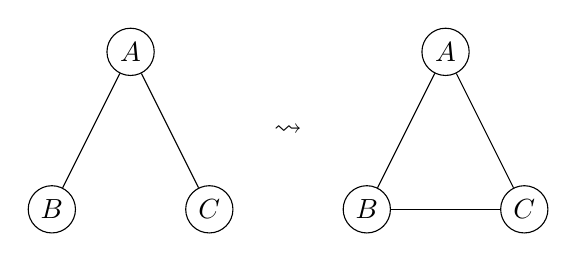
\begin{tikzpicture}[font=\sffamily]
      \node (A1) at (-2,2) {$A$}; 
      \node (B1) at (-3,0) {$B$}; 
      \node (C1) at (-1,0) {$C$}; 
      \node[draw=none] (leadsto) at (0,1) {$\leadsto$};
      \node (A) at (2,2) {$A$}; 
      \node (B) at (1,0) {$B$}; 
      \node (C) at (3,0) {$C$}; 
      \foreach \a/\b in {A1/B1,A1/C1,A/B,B/C,A/C}
        \draw (\a) -- (\b);
    \end{tikzpicture}
\end{document}
